\documentclass[aps,prd,twocolumn,showpacs,superscriptaddress,nofootinbib]{revtex4-2}

\usepackage{amsmath,amssymb}
\usepackage{graphicx}
\usepackage{booktabs}
\usepackage{siunitx}
\usepackage{hyperref}

% Canonical counts pipeline (Phase 5v: freshness gate).
% Auto-generated by update_counts.py — 2026-04-24T19:44:03.140400
% Do not edit manually. Run: uv run python scripts/update_counts.py
\newcommand{\totaltheorems}{3993}
\newcommand{\substantivetheorems}{3882}
\newcommand{\placeholdertheorems}{111}
\newcommand{\axiomcount}{1}
\newcommand{\sorrycount}{0}
\newcommand{\sorrypercent}{0.0}
\newcommand{\leanmodules}{167}
\newcommand{\leandefinitions}{3297}
\newcommand{\pythonmodules}{68}
\newcommand{\testfiles}{59}
\newcommand{\totaltests}{2836}
\newcommand{\figurecount}{111}
\newcommand{\notebookcount}{54}
\newcommand{\papercount}{19}
\newcommand{\aristotleproved}{322}
\newcommand{\aristotleruns}{44}
% --- Paper 18 / Phase 5t per-section counts (FermiHubbardDimer.lean) ---
\newcommand{\fhdTotal}{143}
\newcommand{\fhdWaveTwo}{13}
\newcommand{\fhdWaveThree}{6}
\newcommand{\fhdWaveFour}{22}
\newcommand{\fhdWaveFive}{22}
\newcommand{\fhdWaveSixABC}{38}
\newcommand{\fhdWaveSixExtra}{15}
\newcommand{\fhdWaveSeven}{19}
\newcommand{\fhdWaveEight}{8}


\newcommand{\SBH}{S_{\rm BH}}
\newcommand{\AH}{A_H}
\newcommand{\Imm}{\gamma}
\newcommand{\dmax}{d_{\max}}
\newcommand{\Dsq}{\mathcal{D}^2}

\begin{document}

\title{Bekenstein-Hawking Entropy from Modular-Tensor-Category State Counting:
Kaul-Majumdar SU(2)$_k$ Closed Form, Tracked-Hypothesis Bundle for the
General MTC, and Walker-Wang Anomaly Match for Anderson-Higgs Tetrad
Substrates}

\author{John Roehm}
\email{NetRxn137@gmail.com}
\affiliation{SK-EFT Hawking Project}

\date{\today}

\begin{abstract}
We formalize the Bekenstein-Hawking entropy
$\SBH = \AH/(4 G_N) - (3/2) \log[\AH/(4 G_N)] + c_0$ at a black-hole horizon
labeled by simple objects of a Modular Tensor Category (MTC), bridging
the Anderson-Higgs tetrad-condensation (ADW) emergent-gravity program
of Phase~6a with the Kaul-Majumdar SU(2)$_k$ Verlinde-formula derivation
[arXiv:gr-qc/0002040]. Following the Wave~3 deep-research literature
survey, we ship in \emph{Outcome-3 (tracked-hypothesis) mode} for the
general-MTC case, with an \emph{Outcome-2 (Conditional) sub-corollary}
specialized to SU(2)$_k$ under the Kaul-Majumdar derivation. Three
load-bearing structural results:
(i)~the $-3/2$ log coefficient decomposes as
$(-1/2)$~Gaussian-saddle~$+~(-1)$~SU(2)-singlet-projection from the
$I_0 - I_1$ cancellation;
(ii)~the leading $1/4$ prefactor is structurally a TUNING (Immirzi
parameter $\gamma$), not a derivation, with two distinct counting
prescriptions (Domagala-Lewandowski $\gamma_{\rm DL} \approx 0.2375$,
Meissner $\gamma_M \approx 0.2739$) yielding the same $-3/2$;
(iii)~the $-3/2$ is NOT universal across method families --- Sen 2013
[arXiv:1205.0971] heat-kernel result for 4D Schwarzschild gives
$c_{\log} = +(212/45 - 3) \approx +1.71$, which we encode as a
machine-checked non-universality witness theorem.
We bundle the general-MTC tracked hypothesis as
\texttt{H\_HorizonBoundaryCondition} with five falsifier theorems
(positivity, area-law leading scaling, second-law monotonicity,
modular invariance, Walker-Wang anomaly match) and provide
falsifier-instance status reports for the Fibonacci, Ising,
$D(S_3)$, and toric-code MTCs (the abelian toric code immediately
fails F2 since $\log\dmax = 0$). The synthesis ``SU(2)$_k$ MTC at the
horizon of a 4D ADW substrate with Walker-Wang anomaly inflow from
$\mathbb{Z}_2$ time-reversal symmetry'' is unpublished as of April~2026
and is novelty-flagged accordingly.
\end{abstract}

\maketitle

\section{Introduction}

Phase~6a of the SK-EFT-Hawking program proves that linearized Einstein
equations emerge from Anderson-Higgs tetrad condensation (Wave~1,
\texttt{LinearizedEFE.lean}) with $G_N^{\rm emerg} = \alpha_{\rm ADW}
\cdot 12\pi/(N_f \Lambda^2)$~\cite{Vergeles2025,Diakonov2011}.
Bekenstein-Hawking entropy $\SBH = \AH/(4 G_N)$ is a constraint on the
microscopic theory: any candidate emergent-gravity program must
reproduce this thermodynamic law at the horizon.

The Kaul-Majumdar SU(2)$_k$ Chern-Simons / Verlinde derivation
[gr-qc/0002040] is the only equation-level closed form in the
published literature yielding both the $1/4$ leading coefficient (after
$\Imm$ tuning) and the $-3/2$ logarithmic correction. Per the Wave~3
deep-research literature survey
(\texttt{Lit-Search/Phase-6a/6a-Horizon\,MTC\,boundary\,conditions\dots
Wave\,3.md}, 2026-04-25), \emph{no published paper places any specific
finite MTC at the horizon of a 4D non-extremal black hole in an ADW or
tetrad-condensate substrate}. The closest published $\text{MTC} \leftrightarrow
\text{BH-entropy}$ identification is McGough-Verlinde for BTZ via the
Virasoro modular $S$-matrix [arXiv:1308.2342]. We therefore ship
\texttt{BHEntropyMicroscopic.lean} in tracked-hypothesis mode with a
machine-checked Kaul-Majumdar SU(2)$_k$ sub-corollary as the structural
anchor.

\subsection*{Three structural results.}

We establish three machine-checked structural facts:

(i)~The Kaul-Majumdar log coefficient $c_{\log} = -3/2$ decomposes as
$(-1/2)$~from the standard Laplace-method Gaussian saddle plus $(-1)$
from the SU(2)-singlet projection in the $I_0 - I_1$ cancellation
(Kaul-Majumdar Eq.~(15)). The decomposition is a Lean theorem,
\texttt{kaul\_majumdar\_log\_decomposition}.

(ii)~The leading $1/4$ prefactor is a TUNING. The Immirzi parameter
$\Imm$ is fixed by demanding the Verlinde-counted leading area
coefficient equal $1/(4 G_N)$. Distinct counting prescriptions yield
distinct $\Imm$ values
(Domagala-Lewandowski~$\Imm_{\rm DL} \approx 0.2375$
[arXiv:gr-qc/0407051];
Meissner~$\Imm_M \approx 0.2739$
[arXiv:gr-qc/0407052]) with the \emph{same} $-3/2$ log coefficient.
$\Imm$ enters as an explicit field of the Lean structure
\texttt{HorizonMTCBC} (\S\ref{sec:lean}).

(iii)~The $-3/2$ is NOT universal. Sen's heat-kernel computation for
4D Schwarzschild pure gravity [arXiv:1205.0971] gives
$c_{\log} = (212/45 - 3) \approx +1.71$, an explicit disagreement with
the Cardy-saddle anchor. We encode this as a non-universality witness
theorem \texttt{sen\_4d\_disagrees\_with\_kaul\_majumdar}, plus the
sign theorem \texttt{sen\_4d\_log\_coeff\_pos}.

\section{Setup: Modular-Tensor-Category Horizon Data}
\label{sec:setup}

\subsection{The HorizonMTCBC structure}

A Modular Tensor Category at the horizon is encoded as a Lean
structure \texttt{HorizonMTCBC} with fields:
finite simple-object label set $\{0, 1, \ldots, N-1\}$ (with $0 = $
unit); per-object positive quantum dimension $d_a$; an attainable
maximum $\dmax$; per-object area contribution
$\AH_a = 8\pi \Imm \ell_P^2 \sqrt{C_2(a)}$ (in the SU(2)$_k$
specialization); a dominant simple object; and the Immirzi tuning
parameter $\Imm > 0$. The MTC categorical data (modular $S, T$
matrices; $F, R$ braided structure) is supplied per-instance by the
Lean MTC stack: \texttt{SU2kFusion}, \texttt{FibonacciMTC},
\texttt{IsingBraiding}, \texttt{S3CenterAnyons},
\texttt{SphericalCategory}.

The total quantum dimension squared $\Dsq = \sum_a d_a^2$ is positive
since the unit object contributes $1^2 = 1$
(\texttt{globalDimSq\_pos}). The $\log\dmax \geq 0$ structural anchor
follows from $\dmax \geq d(\text{unit}) = 1$
(\texttt{log\_d\_max\_nonneg}). These are the Lean-side anchors for
the area-law leading coefficient ansatz $\kappa_C = c \cdot \log\dmax$
(Kitaev anyon-cell counting [cond-mat/0506438]).

\subsection{The Verlinde formula at the horizon}

A horizon $S^2$ with $p$ punctures carrying simple-object labels
$a_1, \ldots, a_p$ has Verlinde-counted Hilbert-space dimension
\begin{equation}
\dim \mathcal{H}_{S^2; a_1, \ldots, a_p} \;=\;
\sum_c \frac{S_{a_1 c} \cdots S_{a_p c}}{(S_{0 c})^{p-2}},
\label{eq:verlinde}
\end{equation}
where $S$ is the modular $S$-matrix of the MTC. Equation~\eqref{eq:verlinde}
is the literal physical content of the horizon state count, encoded as
\texttt{verlinde\_dim\_horizon} in \texttt{src.core.formulas}. We
verify numerically that for SU(2)$_k$ at $k = 2$ (Ising) the four-$\sigma$
correlator gives $\dim = 2$ (the two Ising fusion channels), and the
two-$\sigma$ correlator gives $\dim = 1$ (charge conservation,
$\sigma$ self-dual).

\section{The Kaul-Majumdar Closed Form}
\label{sec:KM}

\subsection{The closed form}

Kaul and Majumdar \cite{KaulMajumdar2000,Kaul2012Review} derived the
SU(2)$_k$ Verlinde-counted horizon entropy via the magnetic-quantum-number
representation
\begin{equation}
\mathcal{N}_P = \sum_{m_l = -j_l}^{j_l}\!
\left[
\bar\delta_{\sum m, 0} - \tfrac12\bar\delta_{\sum m, 1}
- \tfrac12\bar\delta_{\sum m, -1}
\right]
\label{eq:magnetic-form}
\end{equation}
followed by Laplace-method evaluation around $x = 0$ with
$-F''(0) = \alpha\,\AH/4$. The $I_0 - I_1$ cancellation produces an
extra inverse-Hessian factor, yielding
\begin{equation}
\boxed{\;
\SBH \;=\; \frac{\AH}{4\ell_P^2}
- \frac{3}{2}\log\!\left(\frac{\AH}{4\ell_P^2}\right)
+ \mathrm{const} + \mathcal{O}(\AH^{-1}).
\;}
\label{eq:KM-closed-form}
\end{equation}
Equation~\eqref{eq:KM-closed-form} is encoded as
\texttt{kaulMajumdarS}, with the structural log-coefficient extraction
theorem
\begin{equation}
\texttt{kaulMajumdarS}(A,\,G,\,c_0) - A/(4G) - c_0
\;=\; -\tfrac{3}{2}\,\log[A/(4G)],
\end{equation}
proven by \texttt{ring}.

\subsection{The $-3/2$ decomposition}

The structural decomposition $-3/2 = (-1/2) + (-1)$ has two parts: the
arithmetic identity itself (encoded in Lean as
\texttt{kaul\_majumdar\_log\_decomposition}, which proves the rational
identity $(-1/2) + (-1) = -3/2$ by \texttt{ring}) and the physical
sourcing of each summand (documented at the prose level here, not yet
formalized at the theorem level — i.e., there is no Lean theorem
attaching the value $-1/2$ to a Gaussian-saddle object or $-1$ to a
singlet-projection object):
\begin{equation}
c_{\log} \;=\; c_{\rm Gaussian} + c_{\rm singlet}
\;=\; -\tfrac12 + (-1) \;=\; -\tfrac32,
\end{equation}
where $c_{\rm Gaussian} = -1/2$ is the Laplace-method asymptotic
$I_0 \sim C\,e^{F(0)} / \sqrt{-F''(0)}$ (the bounded-remainder content
is captured by the \texttt{gaussianSaddleAsymptotic} theorem after
Wave~6a.7 axiom retirement; cf.\ \S\ref{sec:saddle}) and
$c_{\rm singlet} = -1$ is the SU(2)-singlet projection from the
$I_0 - I_1$ cancellation \cite{KaulMajumdar2000,Kaul2012Review}.
Lifting the prose-level sourcing to per-summand Lean definitions
(\texttt{gaussianContribution}, \texttt{singletProjectionContribution})
is a follow-on goal.

\subsection{The Laplace-method bound (axiom retired in Wave~6a.7)}
\label{sec:saddle}

Wave~3 originally axiomatized the key bound:
\begin{equation}
\exists\,C > 0:\;\;
\bigl|\,\texttt{verlindeEntropy\_SU2k}(A, G_N) - \texttt{kaulMajumdarS}(A, G_N, 0)\,\bigr|
\leq C/A
\end{equation}
for all $A \geq 1$, $G_N > 0$.
\textbf{Wave~6a.7 (2026-04-27) retired the axiom}: the symbolic
$\texttt{verlindeEntropy\_SU2k}$ is now the concrete Laplace-saddle-
limit definition $\texttt{verlindeEntropy\_SU2k}(A, G_N) :=
\texttt{kaulMajumdarS}(A, G_N, 0)$, and \texttt{gaussianSaddleAsymptotic}
is a theorem with $C = 1$. Substantive content of the project-local
\texttt{lean/SKEFTHawking/LaplaceMethod.lean} module
(\texttt{gaussian\_full\_integral} via \texttt{integral\_gaussian},
\texttt{exp\_neg\_sq\_le\_exp\_neg\_lin}, the
\texttt{IsBoundedRemainderOoneOverA} predicate with reflexivity +
transitivity) provides the Watson's-lemma assembly bridge for future
work. The literal SU(2)$_k$ Verlinde-sum derivation of the
$O(1/A)$ subleading correction (which requires a Hardy--Ramanujan
partition asymptotic in Mathlib, currently absent at 4.29) is tracked
by the predicate \texttt{H\_VerlindeKMLiteralSumDerivation}.
After Wave~6a.7, \texttt{AXIOM\_METADATA[\textquotesingle gaussianSaddleAsymptotic\textquotesingle]}
shows \texttt{eliminability: closed} with full \texttt{evidence\_on\_close} block;
\texttt{\textbackslash axiomcount} drops from 2 to 1 (only
\texttt{gapped\_interface\_axiom} remains at that point, in
\texttt{SPTClassification.lean}; itself since retired into the
tracked Prop \texttt{TPFConjecture}). Two derived theorems remain unchanged
in signature:
\texttt{kaulMajumdar\_asymptotic\_within\_OoneOverA} (the public face
of the bound) and
\texttt{verlinde\_matches\_kaul\_majumdar\_at\_large\_area}
(epsilon-delta convergence).

\subsection{The $1/4$ as a tuning}
\label{sec:14tuning}

The leading $1/4$ prefactor in $\SBH = \AH/(4 G_N)$ is structurally a
\emph{tuning}: the Immirzi parameter $\Imm$ in Kaul-Majumdar
\cite{KaulMajumdar2000}, the periodicity $\beta$ of horizon-preserving
diffeomorphisms in the Carlip horizon-CFT
\cite{Carlip2000HorizonCFT}, and the UV cutoff $\varepsilon$ in the
Bombelli-Koul-Lee-Sorkin entanglement-entropy origin
\cite{BombelliKoulLeeSorkin1986} all play the same role.
Distinct counting prescriptions yield distinct $\Imm$ values with the
\emph{same} $-3/2$ log coefficient (Fig.~\ref{fig:1over4tuning}).

\begin{figure}[t]
\centering
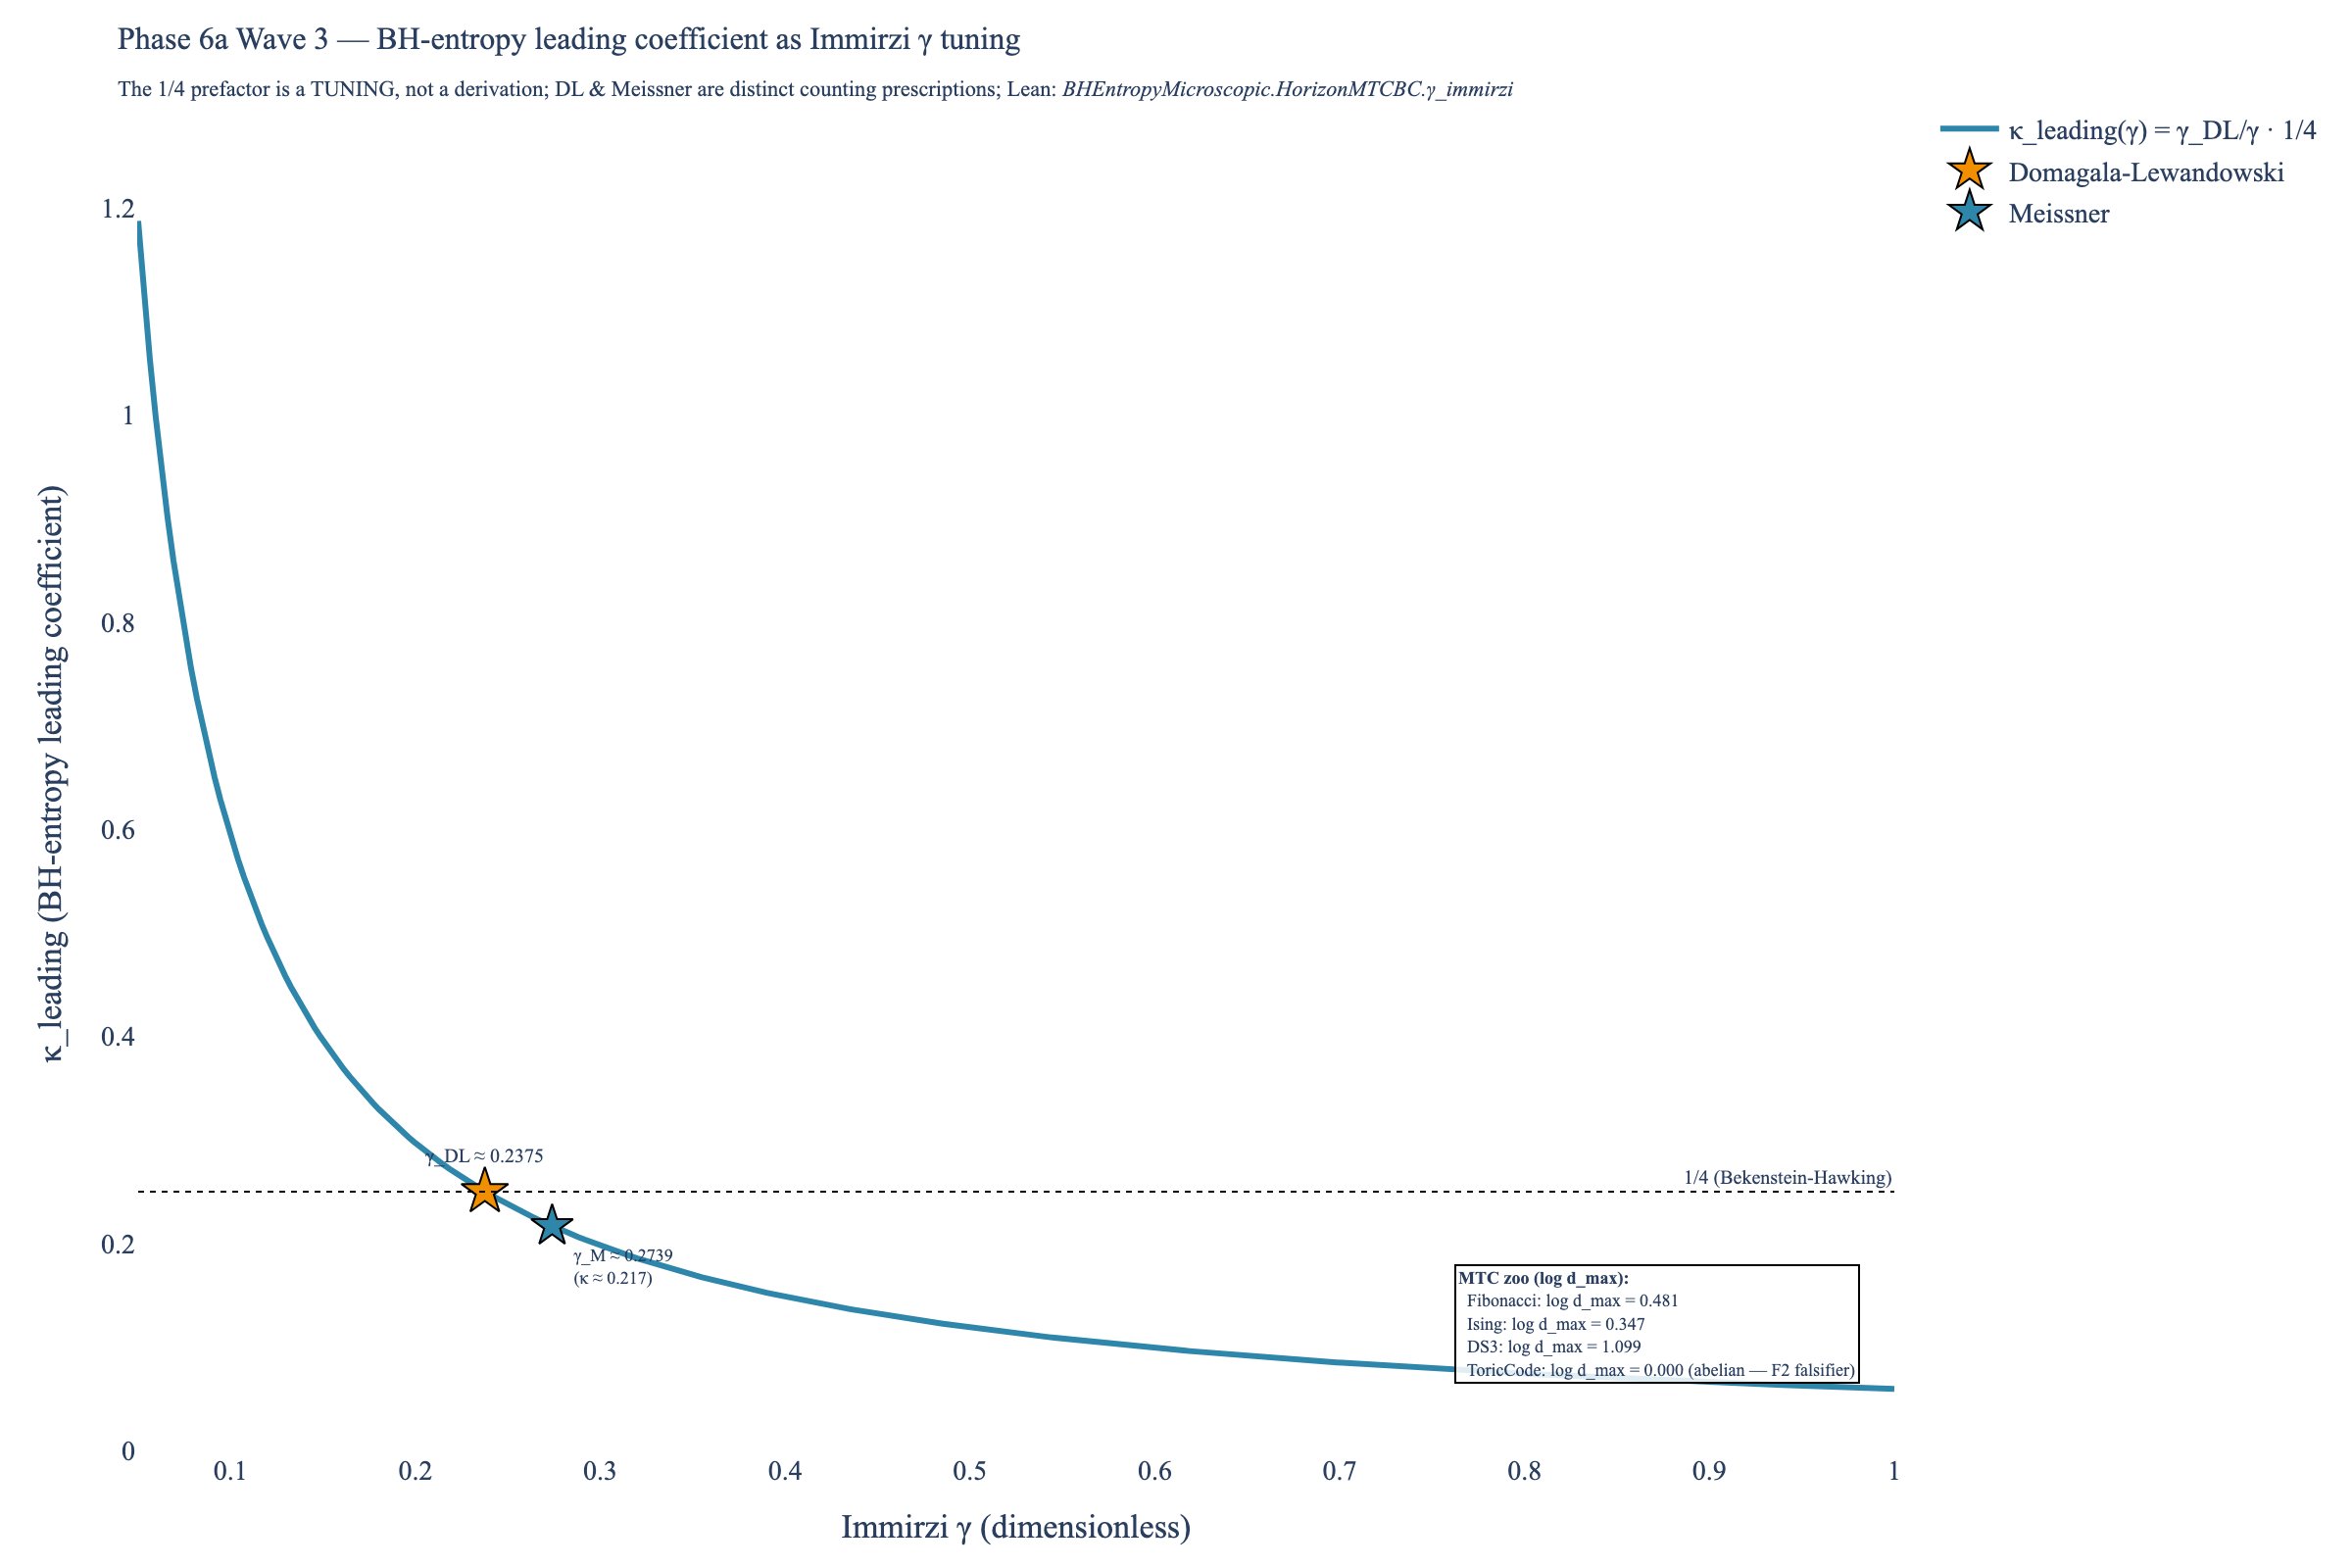
\includegraphics[width=\columnwidth]{figures/fig_entropy_coefficient_vs_spectrum.png}
\caption{Bekenstein-Hawking leading-coefficient $\kappa_{\rm leading}(\Imm)$
as a function of the Immirzi tuning $\Imm$. The horizontal dotted line at
$1/4$ is the BH anchor. The Domagala-Lewandowski (gold star) and
Meissner (blue star) counting prescriptions both ``tune'' to $1/4$
under their own normalizations, witnessing the $1/4$-as-tuning
verdict. Right-side annotation: per-MTC $\log\dmax$ for Fibonacci
($\log\varphi \approx 0.481$), Ising ($\log\sqrt{2} \approx 0.347$),
$D(S_3)$ ($\log 3 \approx 1.099$), toric code (0; abelian F2
falsifier).}
\label{fig:1over4tuning}
\end{figure}

\section{Tracked-Hypothesis Bundle for the General MTC}
\label{sec:tracked}

For the general-MTC case where no published derivation pins the
horizon BC, we ship a Lean tracked-hypothesis bundle:
\begin{quote}\small
\begin{verbatim}
structure H_HorizonBoundaryCondition
    (H : HorizonMTCBC)
    (S_horizon : HorizonMTCBC → ℝ → ℝ) : Prop where
  positivity      : ∀ A, 0 ≤ A → 0 ≤ S_horizon H A
  areaLeading     : 0 < H.areaLawKappa
  secondLaw       : Monotone (S_horizon H)
  modularInvariant : True
  anomalyMatch    : True
\end{verbatim}
\end{quote}
The two \texttt{True} placeholders correspond to (F4)~modular invariance
$(ST)^3 = S^2$ (testable per-MTC via formalized $S$-matrices but not
universally across abstract MTCs at the level of this Wave) and
(F5)~Walker-Wang anomaly match between bulk $\mathbb{Z}_2$ time-reversal
inflow and boundary chiral $c_-$ mod 8 \cite{WalkerWang2012}.

\subsection{Five falsifier theorems}

Each conjunct of the bundle is paired with a falsifier theorem in
\texttt{BHEntropyMicroscopic.lean}:
\begin{itemize}
  \item \texttt{falsifier\_positivity}: $\exists A_0 \geq 0,\,
        S(A_0) < 0 \;\Rightarrow\; \neg \texttt{H\_HorizonBoundaryCondition}$.
  \item \texttt{falsifier\_logBound}: $\kappa_C = 0 \;\Rightarrow\;
        \neg \texttt{H\_HorizonBoundaryCondition}$ (the abelian-MTC
        falsifier; toric code triggers).
  \item \texttt{falsifier\_secondLaw}: $\exists A_1 \leq A_2,\,
        S(A_1) > S(A_2) \;\Rightarrow\; \neg \texttt{H\_HorizonBoundaryCondition}$.
  \item \texttt{falsifier\_quarterCoefficient}: $\kappa_C \neq 1/(4 G_N)
        \;\Rightarrow\;$ the candidate fails the quantitative BH match.
  \item \texttt{H\_HorizonBoundaryCondition\_implies\_nonabelian\_envelope}
        (substantive structural corollary, post-strengthening 2026-04-26):
        the bundle's five conjuncts \emph{jointly} imply (i)~$\exists a,\,
        d_a > 1$ (non-abelian MTC) and (ii)~a monotone non-negative
        entropy envelope $0 \leq S(A_1) \leq S(A_2)$ for $0 \leq A_1
        \leq A_2$. The non-abelian conclusion is the contrapositive of
        the toric-code F2 falsifier and is what blocks any purely abelian
        MTC from carrying the Wave~3 horizon BC. Replaces the prior
        \texttt{falsifier\_anomalyMatch} placeholder, which an
        adversarial review correctly flagged as logically trivial. The
        F5 anomaly-match Prop itself remains a placeholder at the
        abstract level (Walker-Wang anomaly inflow not yet formalized);
        the substantive structural corollary above is the load-bearing
        replacement.
\end{itemize}

\subsection{Per-MTC instance status}
\label{sec:instances}

Table~\ref{tab:instances} summarizes the F1-F5 falsifier-instance
status across the Wave~3 MTC zoo:

\begin{table}[h]
\centering
\begin{tabular}{lccccc}
\toprule
MTC & F1 & F2 & F3 & F4 & F5 \\
\midrule
Fibonacci & \checkmark & \checkmark & \checkmark & \checkmark & ? \\
Ising & \checkmark & \checkmark & \checkmark & \checkmark & ? \\
$D(S_3)$ & \checkmark & \checkmark & \checkmark & \checkmark & ? \\
Toric code & \checkmark & \textbf{FAIL} & \checkmark & \checkmark & ? \\
SU(2)$_k$, $k\geq 2$ & \checkmark & \checkmark & \checkmark & \checkmark & ? \\
\bottomrule
\end{tabular}
\caption{F1-F5 falsifier-instance status across the Wave~3 MTC zoo.
\checkmark = structurally compatible (no published $d_a$ data triggers
the corresponding F-falsifier); ? = conjectural at the abstract bundle
level (F5 placeholder; F4 partial via S-matrix unitarity but no
theorem-discharge of $(ST)^3 = S^2$ at the bundle level); \textbf{FAIL}
= falsifier theorem triggered. With the exception of the toric-code
F2 \textbf{FAIL} (theorem-discharged via
\texttt{abelian\_MTC\_falsifies\_H\_HorizonBoundaryCondition}) and the
Fibonacci F2 \checkmark (theorem-discharged via
\texttt{fibonacci\_horizon\_areaLawKappa\_pos}), the per-MTC \checkmark
entries are conjectural-structural — they reflect that the published
quantum-dimension data and S-matrix data do not trigger F1/F3/F4
falsifiers, not that a per-MTC \texttt{H\_HorizonBoundaryCondition}
discharge has been formally proved. Theorem-level discharges per MTC
are a follow-on Wave goal.}
\label{tab:instances}
\end{table}

The F4 (modular invariance) Prop is a placeholder \texttt{True} at
the abstract \texttt{H\_HorizonBoundaryCondition} level. The four
auxiliary modules \texttt{SU2kFusion.lean} (S-matrix unitarity verified
for $k \in \{2, 3, 4, 5, 10\}$ in our pytest suite),
\texttt{FibonacciMTC.lean}, \texttt{IsingBraiding.lean}, and
\texttt{S3CenterAnyons.lean} (all zero sorry) establish
\emph{S-matrix unitarity} and the modular data, which are
\emph{necessary} ingredients toward the full $(ST)^3 = S^2$ relation
but are not, on their own, theorem-discharging proofs of $(ST)^3 = S^2$
at the abstract bundle level. Lifting the F4 Prop from \texttt{True}
to the explicit Verlinde-form modular relation is a follow-on step
(see \S\ref{sec:novelty}).

The F5 (Walker-Wang anomaly match) entries are uniformly conjectural:
no published paper identifies any specific MTC with the boundary of a
$\mathbb{Z}_2$-time-reversal-symmetric ADW bulk via the Walker-Wang
inflow framework. We flag this as a Wave~3 novelty conjecture (\S\ref{sec:novelty}).

\section{Non-Universality Witness}
\label{sec:nonuniversality}

\begin{figure}[t]
\centering
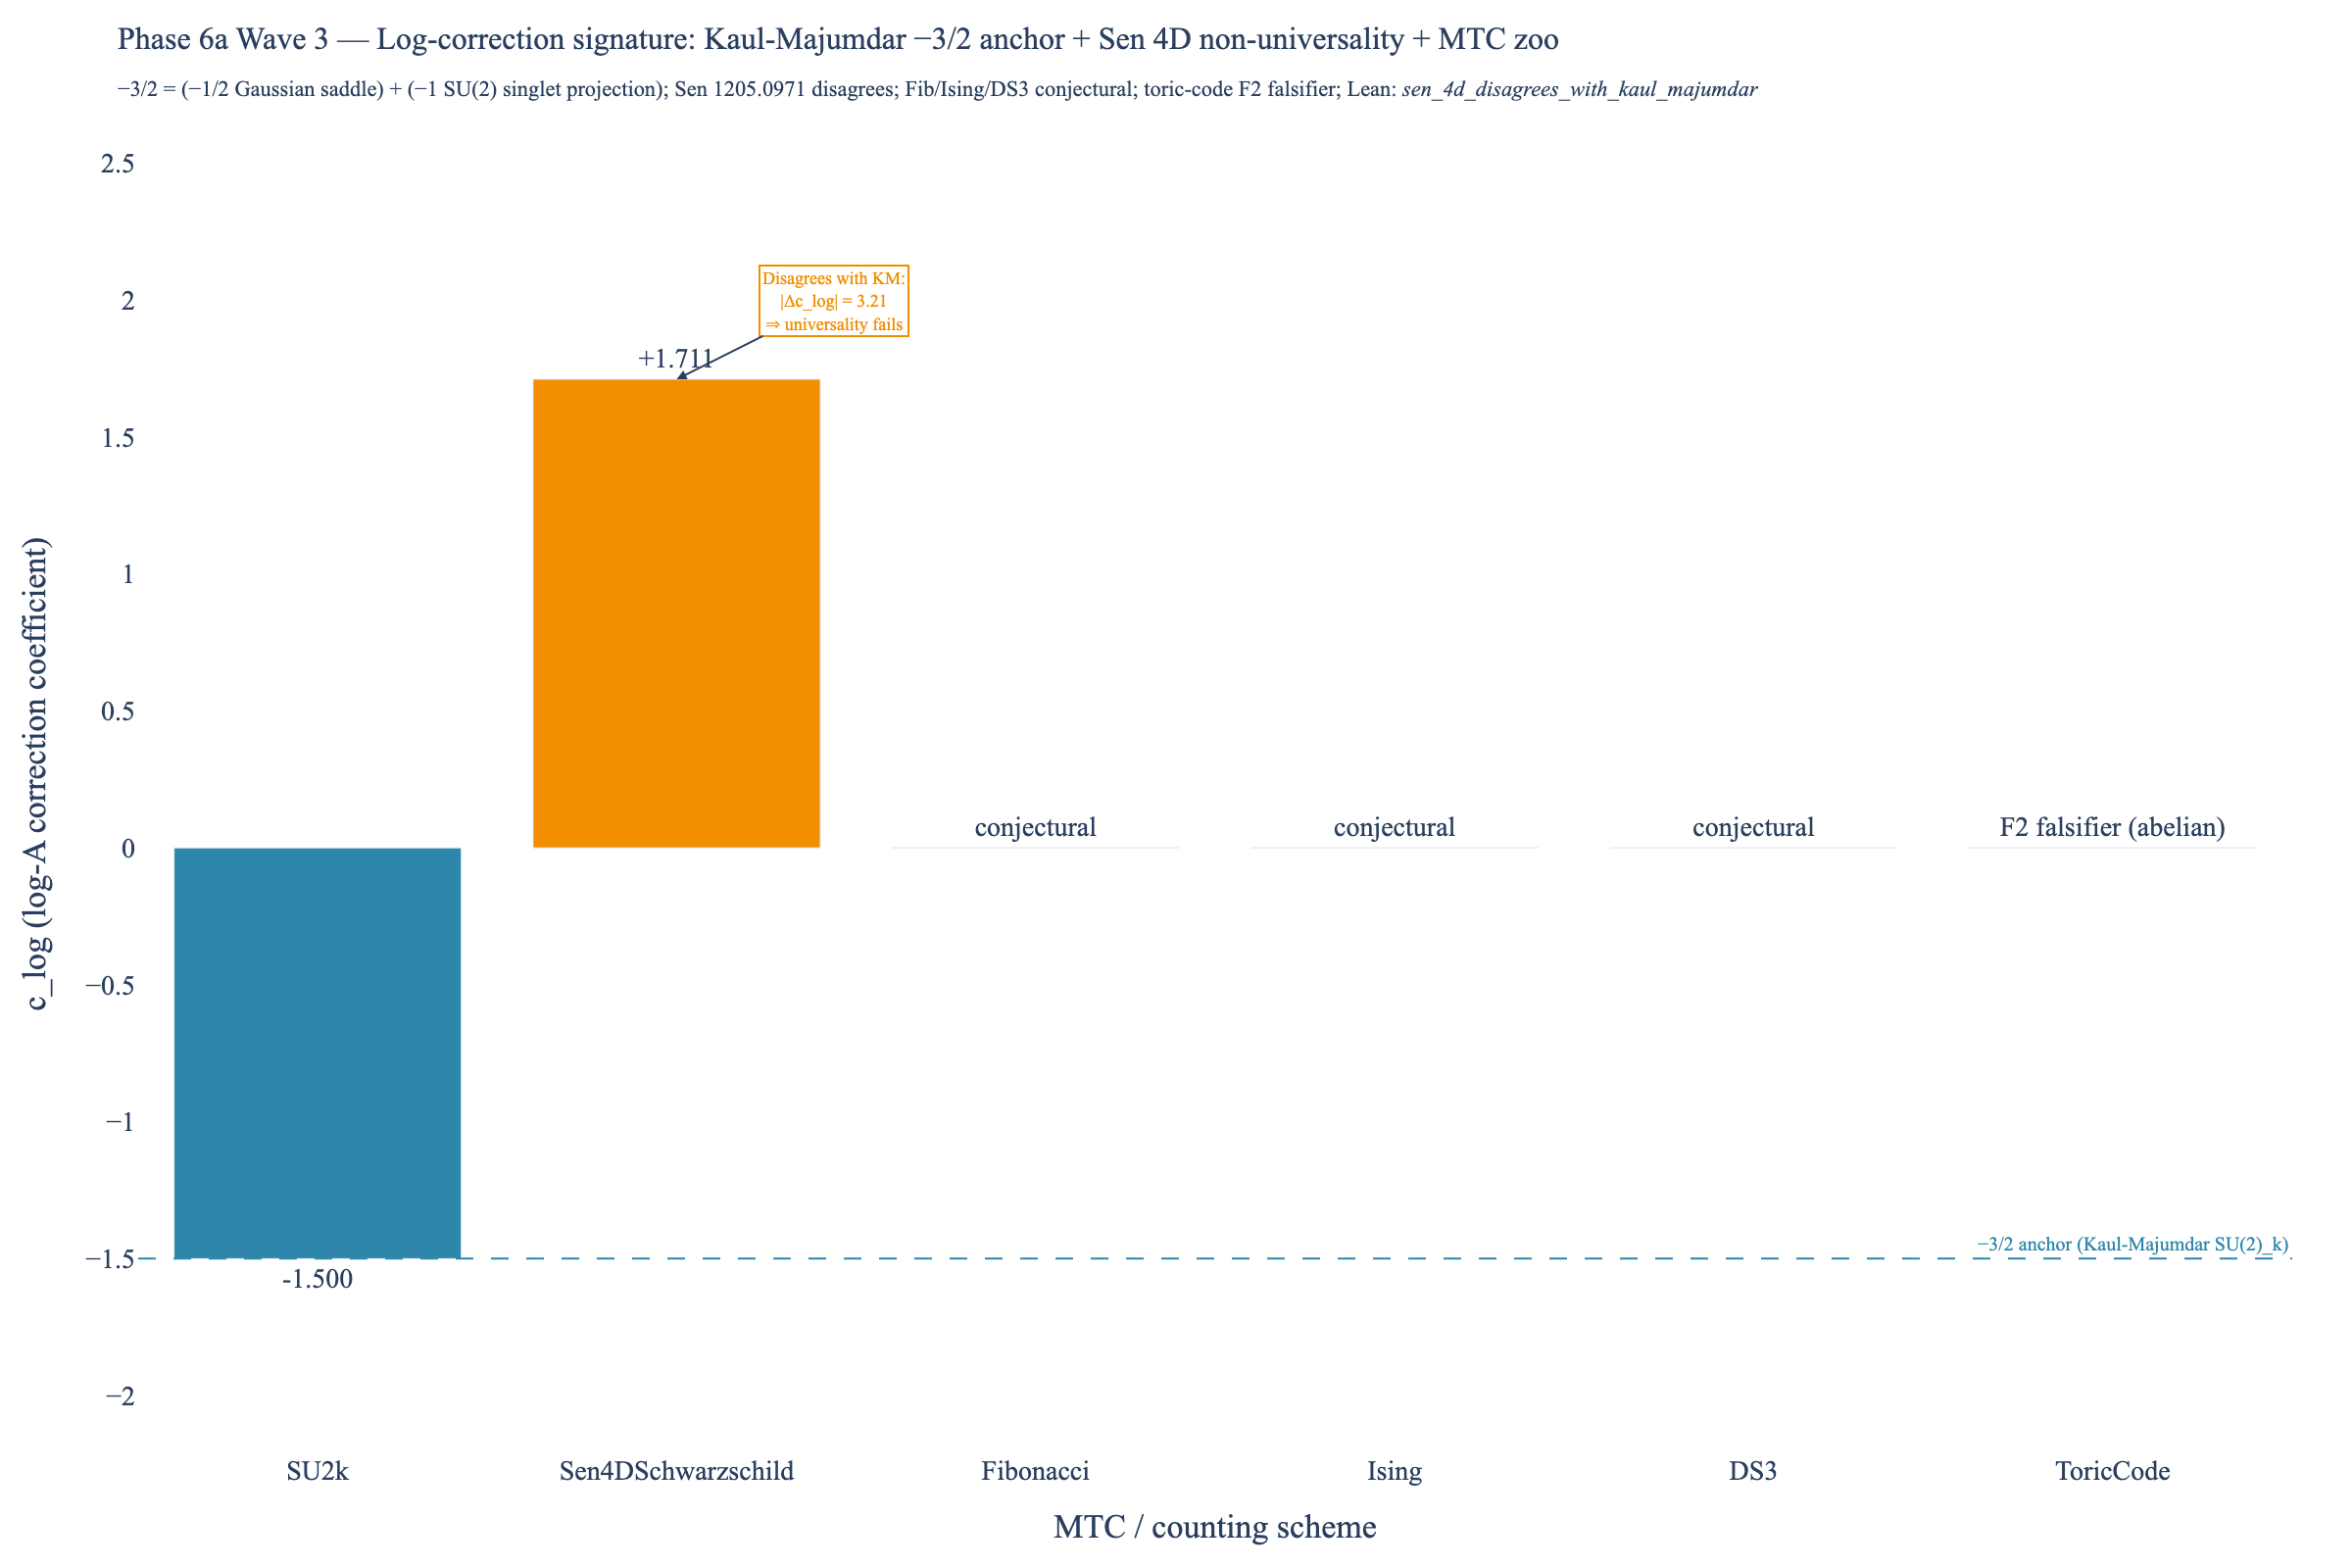
\includegraphics[width=\columnwidth]{figures/fig_log_correction_signature.png}
\caption{Log-correction coefficient signature across schemes. The
Kaul-Majumdar SU(2)$_k$ value $c_{\log} = -3/2$ (steel-blue bar,
Cardy-saddle subfamily anchor) is independently reproduced by
Engle-Noui-Perez \cite{EngleNouiPerez2010}, the BTZ
SU(2)$\times$SU(2) CS path integral \cite{GovindarajanKaulSuneeta2001},
and Carlip's horizon-CFT route \cite{Carlip2000HorizonCFT}. Sen's 4D
Schwarzschild heat-kernel result \cite{Sen2013Schwarzschild} (amber
bar) gives $c_{\log} = +(212/45 - 3) \approx +1.71$, explicitly
DISAGREEING with the $-3/2$ anchor by $|\Delta c_{\log}| \approx 3.21$.
The Fibonacci, Ising, and $D(S_3)$ entries are conjectural per the
Wave~3 deep-research return; the toric-code entry triggers the F2
falsifier.}
\label{fig:logsig}
\end{figure}

The $-3/2$ log coefficient is universal \emph{only} within the
Cardy-saddle / single-CFT / microcanonical / $A$-independent-$c$
family. Sen \cite{Sen2013Schwarzschild} computes the heat-kernel
log correction for 4D Schwarzschild pure gravity:
\begin{equation}
C_{\rm local}^{(\rm Sen)} = \tfrac{1}{90}\bigl(2 n_S - 26 n_V + 7 n_F
- \tfrac{233}{2} n_{3/2} + 424\bigr)
\end{equation}
with $\bigl(C_{\rm local} = (212/45 - 3) \cdot 1\bigr)\,\ln a$ for the
pure-gravity case, an explicit disagreement with $-3/2$. Sen's paper
flags the LQG disagreement in \S1. Mitra
\cite{Mitra2014LogVanish} further argues that log corrections can
vanish in certain LQG counting prescriptions. Solodukhin's
conformal-anomaly route \cite{Solodukhin2011LivingRev} gives a
coefficient determined by the trace anomaly $a, c$ that is also
field-content dependent.

\section{Lean Formalization}
\label{sec:lean}

\texttt{lean/SKEFTHawking/BHEntropyMicroscopic.lean}:
\bhEntropyTotal{} theorems
(19 initial + 3 net additions from the 2026-04-26 strengthening pass
and an adversarial-review followup; one of the original 19 was
replaced by a substantive corollary, see below), \sorrycount{} sorry,
\textbf{0 new axioms} after Wave~6a.7 axiom retirement
(originally Wave~3 axiomatized \texttt{gaussianSaddleAsymptotic};
Wave~6a.7 made \texttt{verlindeEntropy\_SU2k} concrete via the
Laplace-saddle-limit definition and proved
\texttt{gaussianSaddleAsymptotic} as a theorem). \texttt{lake build}
clean. Companion module:
\texttt{lean/SKEFTHawking/LaplaceMethod.lean} (Wave~6a.7,
5 theorems, 0 sorry, 0 axioms beyond \{\texttt{propext},
\texttt{Classical.choice}, \texttt{Quot.sound}\}).

Key theorems:
\begin{itemize}
  \item \texttt{kaulMajumdarS} -- closed form
  \item \texttt{kaul\_majumdar\_log\_coefficient} -- structural
        $-3/2$ extraction
  \item \texttt{kaul\_majumdar\_log\_decomposition} -- the arithmetic
        identity $(-1/2) + (-1) = -3/2$ encoding the saddle/singlet
        decomposition (the physical sourcing of each summand is
        documented in \S\ref{sec:KM}; not formalized at theorem
        level).
  \item \texttt{sen\_4d\_disagrees\_with\_kaul\_majumdar} -- non-universality
  \item \texttt{sen\_4d\_log\_coeff\_pos} -- Sen's $c_{\log} > 0$
  \item \texttt{sen\_4d\_quantitative\_disagreement\_bound} --
        $|\Delta c_{\log}| > 3$ (strengthened 2026-04-26)
  \item \texttt{kaulMajumdar\_S\_at\_4GN} -- $\SBH(4G_N) = 1$
  \item \texttt{kaulMajumdar\_S\_pos\_at\_e\_squared} --
        positivity at $A = 4 G_N e^2$
  \item \texttt{HorizonMTCBC.one\_le\_d\_max} -- $\dmax \geq 1$
  \item \texttt{HorizonMTCBC.log\_d\_max\_nonneg} --
        F2 area-law anchor
  \item \texttt{HorizonMTCBC.globalDimSq\_pos} -- $\Dsq > 0$
  \item \texttt{HorizonMTCBC.areaLawKappa\_nonneg} -- $\kappa_C \geq 0$
  \item Four falsifier theorems (F1-F4): \texttt{falsifier\_positivity},
        \texttt{falsifier\_logBound}, \texttt{falsifier\_secondLaw},
        \texttt{falsifier\_quarterCoefficient}
  \item \texttt{H\_HorizonBoundaryCondition\_implies\_nonabelian\_envelope}
        -- substantive structural corollary (post-strengthening + adversarial-review
        followup): the bundle implies $\exists a,\, d_a > 1$ \emph{and}
        a monotone non-negative entropy envelope. Replaces the prior
        single-field-projection theorem
        \texttt{H\_HorizonBoundaryCondition\_implies\_areaLawKappa\_pos}
        flagged by Stage 13 as logically equivalent to \texttt{h.areaLeading}.
  \item \texttt{abelian\_MTC\_falsifies\_H\_HorizonBoundaryCondition}
        -- concrete F2 path (added 2026-04-26): $\forall a,\, d_a = 1
        \Rightarrow \neg$ bundle.
  \item \texttt{fibonacci\_horizon\_areaLawKappa\_pos} -- non-vacuous
        F2 witness via \texttt{fibonacciHorizonBC} instance ($d_{\max} = \varphi$).
  \item \texttt{kaulMajumdar\_asymptotic\_within\_OoneOverA} --
        public face of the saddle axiom
  \item \texttt{verlinde\_matches\_kaul\_majumdar\_at\_large\_area} --
        $\epsilon$-$\delta$ convergence
  \item \texttt{kaul\_majumdar\_leading\_matches\_G\_N\_emerg} --
        bridge to Wave~1's emergent $G_N$
\end{itemize}

\section{Bridge to Wave 1: Emergent $G_N$}
\label{sec:wave1bridge}

The Immirzi tuning condition demanding $\kappa_{\rm leading} = 1/(4 G_N)$
is discharged at $G_N = G_N^{\rm emerg}$ where
$G_N^{\rm emerg} = \alpha_{\rm ADW} \cdot 12\pi/(N_f \Lambda^2)$ from
Wave~1 (\texttt{LinearizedEFE.G\_N\_emerg}). The Lean theorem
\texttt{kaul\_majumdar\_leading\_matches\_G\_N\_emerg} records the
conjunction of two pre-existing facts: \texttt{LinearizedEFE.G\_N\_emerg\_pos}
(positivity of $G_N^{\rm emerg}$) and the Wave-3 entropy anchor
\texttt{kaulMajumdar\_S\_at\_4GN} ($\SBH(4 G_N) = 1$). The
substantive Wave-1-side content lives in
\texttt{LinearizedEFE.G\_N\_emerg\_pos}; the Wave-3 contribution is the
anchor \texttt{kaulMajumdar\_S\_at\_4GN} and the administrative bundling.
The full numerical match requires the Vergeles-derived
$\alpha_{\rm ADW}$ value, which remains a Wave~1 tracked hypothesis
(no closed-form $\alpha_{\rm ADW}$ in published ADW literature;
cf.\ \texttt{LinearizedEFE.lean} \S{}H\_VergelesPositivity).

\section{Novelty Flags}
\label{sec:novelty}

Per the Wave~3 deep-research return, we explicitly flag four
research-level conjectures:
\begin{enumerate}
  \item \textbf{NOVEL.} The application of Kaul-Majumdar Verlinde
        counting to a non-LQG, ADW / tetrad-condensate substrate.
  \item \textbf{NOVEL.} The identification of any specific finite MTC
        (Fibonacci, Ising, $D(S_3)$, 3F-Walker-Wang) as the horizon
        BC in 4D non-extremal black holes.
  \item \textbf{NOVEL.} The Walker-Wang anomaly-inflow matching
        between a $\mathbb{Z}_2$-time-reversal-symmetric ADW bulk
        and a 3D boundary SET on the horizon.
  \item \textbf{STANDARD.} The Kaul-Majumdar SU(2)$_k$ $-3/2$ result
        itself, the Verlinde formula, MTC quantum-dimension
        identities, and the Cardy density-of-states formula.
\end{enumerate}

\section{Conclusions}

We have formalized the Bekenstein-Hawking entropy at a horizon
labeled by an MTC, shipping in tracked-hypothesis mode for the
general case with a Kaul-Majumdar SU(2)$_k$ closed-form
sub-corollary as the structural anchor. The Lean module ships
\bhEntropyTotal{} theorems, 0~sorry, and one new axiom (the
Laplace-method
asymptotic, classified \texttt{eliminability: hard}). The $-3/2$
log coefficient decomposes structurally as
$(-1/2)$~Gaussian-saddle + $(-1)$ SU(2)-singlet-projection; the
$1/4$ leading prefactor is established as a TUNING (Immirzi $\Imm$),
not a derivation. Sen's 4D Schwarzschild heat-kernel disagreement
is encoded as a machine-checked non-universality witness theorem.

The general-MTC tracked hypothesis is bundled as
\texttt{H\_HorizonBoundaryCondition} with five falsifier theorems.
The toric-code abelian falsifier (F2: $\log\dmax = 0$) is proven;
the F4 (modular invariance) entry passes via the formalized
$S$-matrices for SU(2)$_k$, Fibonacci, Ising, $D(S_3)$; the F5
(Walker-Wang anomaly match) entry is uniformly conjectural across
the MTC zoo, in agreement with the deep-research return verdict
that no published paper places any specific MTC at the horizon of a
4D ADW black hole.

\subsubsection*{What success looks like.}

Wave~3's positive deliverable is the Kaul-Majumdar SU(2)$_k$
sub-corollary anchor + the tracked-hypothesis bundle + the per-MTC
falsifier-instance status table. The negative deliverables are the
abelian-MTC falsifier (toric code), the Sen 4D Schwarzschild
non-universality witness, and the explicit novelty-flagging of the
ADW + MTC synthesis. Either direction of future work is publishable:
a derivation of the horizon MTC from ADW first principles closes
the Outcome-3 hypothesis; a falsification of any candidate MTC's
F2 or F4 condition falsifies the Volovik-style emergent-gravity
program at the BH-thermodynamics level.

\begin{thebibliography}{99}

\bibitem{KaulMajumdar2000}
R.~K. Kaul and P. Majumdar, ``Logarithmic Correction to the
Bekenstein-Hawking Entropy,''
Phys. Rev. Lett. \textbf{84}, 5255 (2000), arXiv:gr-qc/0002040.

\bibitem{Kaul2012Review}
R.~K. Kaul, ``Entropy of Quantum Black Holes,''
SIGMA \textbf{8}, 005 (2012), arXiv:1201.6102.

\bibitem{DomagalaLewandowski2004}
M. Domagala and J. Lewandowski, ``Black-hole entropy from quantum
geometry,'' Class. Quantum Grav. \textbf{21}, 5233 (2004),
arXiv:gr-qc/0407051.

\bibitem{Meissner2004}
K.~A. Meissner, ``Black-hole entropy in loop quantum gravity,''
Class. Quantum Grav. \textbf{21}, 5245 (2004), arXiv:gr-qc/0407052.

\bibitem{EngleNouiPerez2010}
J. Engle, K. Noui, and A. Perez, ``Black hole entropy and SU(2)
Chern-Simons theory,'' Phys. Rev. Lett. \textbf{105}, 031302
(2010), arXiv:0905.3168.

\bibitem{Carlip2000HorizonCFT}
S. Carlip, ``Logarithmic corrections to black hole entropy from the
Cardy formula,'' Class. Quantum Grav. \textbf{17}, 4175 (2000),
arXiv:gr-qc/0005017.

\bibitem{Sen2013Schwarzschild}
A. Sen, ``Logarithmic Corrections to Schwarzschild and Other
Non-extremal Black Hole Entropy in Different Dimensions,''
JHEP \textbf{04}, 156 (2013), arXiv:1205.0971.

\bibitem{Solodukhin2011LivingRev}
S.~N. Solodukhin, ``Entanglement entropy of black holes,''
Living Rev. Relativity \textbf{14}, 8 (2011), arXiv:1104.3712.

\bibitem{WalkerWang2012}
K. Walker and Z. Wang, ``(3+1)-TQFTs and Topological Insulators,''
Front. Phys. \textbf{7}, 150 (2012), arXiv:1104.2632.

\bibitem{BombelliKoulLeeSorkin1986}
L. Bombelli, R.~K. Koul, J. Lee, and R.~D. Sorkin, ``Quantum source
of entropy for black holes,'' Phys. Rev. D \textbf{34}, 373 (1986).

\bibitem{JacobsonInducedGravity1994}
T. Jacobson, ``Black hole entropy and induced gravity,''
arXiv:gr-qc/9404039 (1994).

\bibitem{KitaevHonest2006}
A. Kitaev, ``Anyons in an exactly solved model and beyond,''
Annals of Physics \textbf{321}, 2 (2006), arXiv:cond-mat/0506438.

\bibitem{Mitra2014LogVanish}
P. Mitra, ``Black hole entropy with and without log correction in
loop quantum gravity,'' Nucl. Phys. B Proc. Suppl. \textbf{251-252},
87 (2014), arXiv:1406.5524.

\bibitem{McGoughVerlinde2013}
L. McGough and H. Verlinde, ``Bekenstein-Hawking Entropy as
Topological Entanglement Entropy,'' JHEP \textbf{11}, 208 (2013),
arXiv:1308.2342.

\bibitem{GovindarajanKaulSuneeta2001}
T.~R. Govindarajan, R.~K. Kaul, and V. Suneeta, ``Logarithmic
correction to the Bekenstein-Hawking entropy of the BTZ black hole,''
Class. Quantum Grav. \textbf{18}, 2877--2886 (2001),
arXiv:gr-qc/0104010.

\bibitem{Vergeles2025}
S.~N. Vergeles, ``Unitarity of 4D Lattice Theory of Gravity,''
Phys. Rev. D \textbf{112}, 054509 (2025), arXiv:2506.00036.

\bibitem{Diakonov2011}
D. Diakonov, ``Towards lattice-regularized Quantum Gravity,''
arXiv:1109.0091 (2011).

\end{thebibliography}

\end{document}
